\documentclass[]{article}
\usepackage{lmodern}
\usepackage{amssymb,amsmath}
\usepackage{ifxetex,ifluatex}
\usepackage{fixltx2e} % provides \textsubscript
\ifnum 0\ifxetex 1\fi\ifluatex 1\fi=0 % if pdftex
  \usepackage[T1]{fontenc}
  \usepackage[utf8]{inputenc}
\else % if luatex or xelatex
  \ifxetex
    \usepackage{mathspec}
  \else
    \usepackage{fontspec}
  \fi
  \defaultfontfeatures{Ligatures=TeX,Scale=MatchLowercase}
\fi
% use upquote if available, for straight quotes in verbatim environments
\IfFileExists{upquote.sty}{\usepackage{upquote}}{}
% use microtype if available
\IfFileExists{microtype.sty}{%
\usepackage[]{microtype}
\UseMicrotypeSet[protrusion]{basicmath} % disable protrusion for tt fonts
}{}
\PassOptionsToPackage{hyphens}{url} % url is loaded by hyperref
\usepackage[unicode=true]{hyperref}
\hypersetup{
            pdftitle={Predavanje 08 -- GRASS GIS},
            pdfborder={0 0 0},
            breaklinks=true}
\urlstyle{same}  % don't use monospace font for urls
\usepackage[margin=1in]{geometry}
\usepackage{color}
\usepackage{fancyvrb}
\newcommand{\VerbBar}{|}
\newcommand{\VERB}{\Verb[commandchars=\\\{\}]}
\DefineVerbatimEnvironment{Highlighting}{Verbatim}{commandchars=\\\{\}}
% Add ',fontsize=\small' for more characters per line
\usepackage{framed}
\definecolor{shadecolor}{RGB}{248,248,248}
\newenvironment{Shaded}{\begin{snugshade}}{\end{snugshade}}
\newcommand{\KeywordTok}[1]{\textcolor[rgb]{0.13,0.29,0.53}{\textbf{#1}}}
\newcommand{\DataTypeTok}[1]{\textcolor[rgb]{0.13,0.29,0.53}{#1}}
\newcommand{\DecValTok}[1]{\textcolor[rgb]{0.00,0.00,0.81}{#1}}
\newcommand{\BaseNTok}[1]{\textcolor[rgb]{0.00,0.00,0.81}{#1}}
\newcommand{\FloatTok}[1]{\textcolor[rgb]{0.00,0.00,0.81}{#1}}
\newcommand{\ConstantTok}[1]{\textcolor[rgb]{0.00,0.00,0.00}{#1}}
\newcommand{\CharTok}[1]{\textcolor[rgb]{0.31,0.60,0.02}{#1}}
\newcommand{\SpecialCharTok}[1]{\textcolor[rgb]{0.00,0.00,0.00}{#1}}
\newcommand{\StringTok}[1]{\textcolor[rgb]{0.31,0.60,0.02}{#1}}
\newcommand{\VerbatimStringTok}[1]{\textcolor[rgb]{0.31,0.60,0.02}{#1}}
\newcommand{\SpecialStringTok}[1]{\textcolor[rgb]{0.31,0.60,0.02}{#1}}
\newcommand{\ImportTok}[1]{#1}
\newcommand{\CommentTok}[1]{\textcolor[rgb]{0.56,0.35,0.01}{\textit{#1}}}
\newcommand{\DocumentationTok}[1]{\textcolor[rgb]{0.56,0.35,0.01}{\textbf{\textit{#1}}}}
\newcommand{\AnnotationTok}[1]{\textcolor[rgb]{0.56,0.35,0.01}{\textbf{\textit{#1}}}}
\newcommand{\CommentVarTok}[1]{\textcolor[rgb]{0.56,0.35,0.01}{\textbf{\textit{#1}}}}
\newcommand{\OtherTok}[1]{\textcolor[rgb]{0.56,0.35,0.01}{#1}}
\newcommand{\FunctionTok}[1]{\textcolor[rgb]{0.00,0.00,0.00}{#1}}
\newcommand{\VariableTok}[1]{\textcolor[rgb]{0.00,0.00,0.00}{#1}}
\newcommand{\ControlFlowTok}[1]{\textcolor[rgb]{0.13,0.29,0.53}{\textbf{#1}}}
\newcommand{\OperatorTok}[1]{\textcolor[rgb]{0.81,0.36,0.00}{\textbf{#1}}}
\newcommand{\BuiltInTok}[1]{#1}
\newcommand{\ExtensionTok}[1]{#1}
\newcommand{\PreprocessorTok}[1]{\textcolor[rgb]{0.56,0.35,0.01}{\textit{#1}}}
\newcommand{\AttributeTok}[1]{\textcolor[rgb]{0.77,0.63,0.00}{#1}}
\newcommand{\RegionMarkerTok}[1]{#1}
\newcommand{\InformationTok}[1]{\textcolor[rgb]{0.56,0.35,0.01}{\textbf{\textit{#1}}}}
\newcommand{\WarningTok}[1]{\textcolor[rgb]{0.56,0.35,0.01}{\textbf{\textit{#1}}}}
\newcommand{\AlertTok}[1]{\textcolor[rgb]{0.94,0.16,0.16}{#1}}
\newcommand{\ErrorTok}[1]{\textcolor[rgb]{0.64,0.00,0.00}{\textbf{#1}}}
\newcommand{\NormalTok}[1]{#1}
\usepackage{graphicx,grffile}
\makeatletter
\def\maxwidth{\ifdim\Gin@nat@width>\linewidth\linewidth\else\Gin@nat@width\fi}
\def\maxheight{\ifdim\Gin@nat@height>\textheight\textheight\else\Gin@nat@height\fi}
\makeatother
% Scale images if necessary, so that they will not overflow the page
% margins by default, and it is still possible to overwrite the defaults
% using explicit options in \includegraphics[width, height, ...]{}
\setkeys{Gin}{width=\maxwidth,height=\maxheight,keepaspectratio}
\IfFileExists{parskip.sty}{%
\usepackage{parskip}
}{% else
\setlength{\parindent}{0pt}
\setlength{\parskip}{6pt plus 2pt minus 1pt}
}
\setlength{\emergencystretch}{3em}  % prevent overfull lines
\providecommand{\tightlist}{%
  \setlength{\itemsep}{0pt}\setlength{\parskip}{0pt}}
\setcounter{secnumdepth}{0}
% Redefines (sub)paragraphs to behave more like sections
\ifx\paragraph\undefined\else
\let\oldparagraph\paragraph
\renewcommand{\paragraph}[1]{\oldparagraph{#1}\mbox{}}
\fi
\ifx\subparagraph\undefined\else
\let\oldsubparagraph\subparagraph
\renewcommand{\subparagraph}[1]{\oldsubparagraph{#1}\mbox{}}
\fi

% set default figure placement to htbp
\makeatletter
\def\fps@figure{htbp}
\makeatother


\title{Predavanje 08 -- GRASS GIS}
\author{}
\date{\vspace{-2.5em}}

\begin{document}
\maketitle

\subsection{GRASS GIS z RGrass7}\label{grass-gis-z-rgrass7}


Zaženemo GrassGis iz konzole:

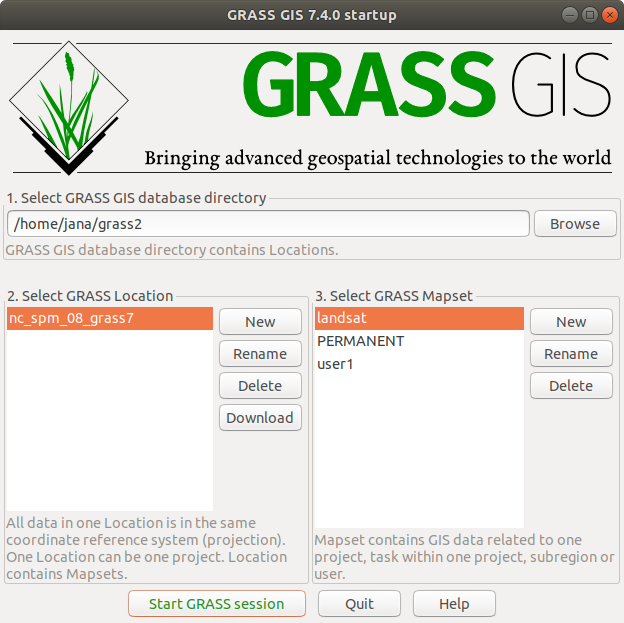
\includegraphics[width=6cm, height=5cm]{/home/jana/git/R-za-neprogramerje/Predavanje_08/grass/grass_gis_gui.png}

V konzoli iz GrassGis-a zaženemo RStudio.

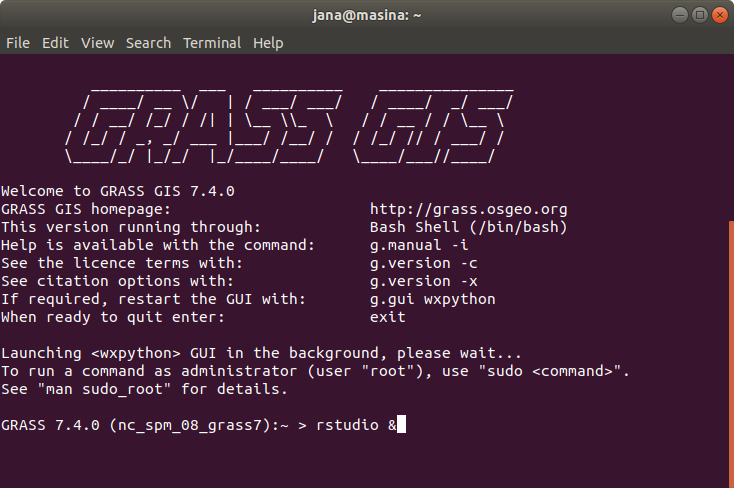
\includegraphics[width=6cm, height=5cm]{/home/jana/git/R-za-neprogramerje/Predavanje_08/grass/Rstudi_zagon.png}

Potrebujemo dve R knjižnici, \textbf{rgrass7} in \textbf{rgdal}.

\begin{Shaded}
\begin{Highlighting}[]
\KeywordTok{library}\NormalTok{(rgrass7)}
\end{Highlighting}
\end{Shaded}

\begin{verbatim}
## Loading required package: XML
\end{verbatim}

\begin{verbatim}
## GRASS GIS interface loaded with GRASS version: GRASS 7.4.0 (2018)
## and location: nc_spm_08_grass7
\end{verbatim}

\begin{Shaded}
\begin{Highlighting}[]
\KeywordTok{library}\NormalTok{(rgdal)}
\end{Highlighting}
\end{Shaded}

\begin{verbatim}
## Loading required package: sp
\end{verbatim}

\begin{verbatim}
## Please note that rgdal will be retired by the end of 2023,
## plan transition to sf/stars/terra functions using GDAL and PROJ
## at your earliest convenience.
## 
## rgdal: version: 1.5-29, (SVN revision 1165M)
## Geospatial Data Abstraction Library extensions to R successfully loaded
## Loaded GDAL runtime: GDAL 2.2.3, released 2017/11/20
## Path to GDAL shared files: /usr/share/gdal/2.2
## GDAL binary built with GEOS: TRUE 
## Loaded PROJ runtime: Rel. 4.9.3, 15 August 2016, [PJ_VERSION: 493]
## Path to PROJ shared files: (autodetected)
## Linking to sp version:1.4-6
\end{verbatim}

Beremo vzorčni primer iz podatkov pridobljenih na
\url{https://grassbook.org/datasets/datasets-3rd-edition/}.

Lahko si pogledamo metapodatke za svojo lokacijo z:

\begin{Shaded}
\begin{Highlighting}[]
\NormalTok{G <-}\StringTok{ }\KeywordTok{gmeta}\NormalTok{()}
\KeywordTok{str}\NormalTok{(G)}
\end{Highlighting}
\end{Shaded}

\begin{verbatim}
## List of 27
##  $ LOCATION_NAME: chr "nc_spm_08_grass7"
##  $ GISDBASE     : chr "/home/jana/grass2"
##  $ MAPSET       : chr "landsat"
##  $ GUI          : chr "wxpython"
##  $ PID          : chr "19616"
##  $ GUI_PID      : chr "19617"
##  $ projection   : chr "99"
##  $ zone         : chr "0"
##  $ n            : num 228500
##  $ s            : num 215000
##  $ w            : num 630000
##  $ e            : num 645000
##  $ t            : num 1
##  $ b            : num 0
##  $ nsres        : num 10
##  $ nsres3       : num 10
##  $ ewres        : num 10
##  $ ewres3       : num 10
##  $ tbres        : num 1
##  $ rows         : int 1350
##  $ rows3        : int 1350
##  $ cols         : int 1500
##  $ cols3        : int 1500
##  $ depths       : int 1
##  $ cells        : chr "2025000"
##  $ cells3       : chr "2025000"
##  $ proj4        : chr "+proj=lcc +lat_1=36.16666666666666 +lat_2=34.33333333333334 +lat_0=33.75 +lon_0=-79 +x_0=609601.22 +y_0=0 +no_d"| __truncated__
##  - attr(*, "class")= chr "gmeta"
\end{verbatim}

Prikaže vektorske zemljevide, ki so na voljo:

\begin{Shaded}
\begin{Highlighting}[]
\KeywordTok{execGRASS}\NormalTok{(}\StringTok{"g.list"}\NormalTok{, }\DataTypeTok{parameters =} \KeywordTok{list}\NormalTok{(}\DataTypeTok{type =} \StringTok{"vector"}\NormalTok{))}
\end{Highlighting}
\end{Shaded}

\begin{verbatim}
## P079214
## P079215
## P079218
## P079219
## boundary_county
## boundary_municp
## bridges
## busroute1
## busroute11
## busroute6
## busroute_a
## busroutesall
## busstopsall
## census_wake2000
## censusblk_swwake
## comm_colleges
## elev_lid792_bepts
## elev_lid792_cont1m
## elev_lid792_randpts
## elev_lidrural_mrpts
## elev_lidrural_mrptsft
## elev_ned10m_cont10m
## firestations
## geodetic_pts
## geodetic_swwake_pts
## geology
## geonames_NC
## geonames_wake
## hospitals
## lakes
## nc_state
## overpasses
## poi_names_wake
## precip_30ynormals
## precip_30ynormals_3d
## railroads
## roadsmajor
## schools_wake
## soils_general
## soils_wake
## streams
## streets_wake
## swwake_10m
## urbanarea
## usgsgages
## zipcodes_wake
\end{verbatim}

Prikaži mrežne zemljevide

\begin{Shaded}
\begin{Highlighting}[]
\KeywordTok{execGRASS}\NormalTok{(}\StringTok{"g.list"}\NormalTok{, }\DataTypeTok{parameters =} \KeywordTok{list}\NormalTok{(}\DataTypeTok{type =} \StringTok{"raster"}\NormalTok{))}
\end{Highlighting}
\end{Shaded}

\begin{verbatim}
## aspect
## basin_50K
## boundary_county_500m
## cfactorbare_1m
## cfactorgrow_1m
## el_D782_6m
## el_D783_6m
## el_D792_6m
## el_D793_6m
## elev_lid792_1m
## elev_ned_30m
## elev_srtm_30m
## elev_state_500m
## elevation
## elevation_shade
## facility
## geology_30m
## lakes
## landclass96
## landcover_1m
## landuse96_28m
## lsat5_1987_10
## lsat5_1987_20
## lsat5_1987_30
## lsat5_1987_40
## lsat5_1987_50
## lsat5_1987_60
## lsat5_1987_70
## lsat7_2000_10
## lsat7_2000_20
## lsat7_2000_30
## lsat7_2000_40
## lsat7_2000_50
## lsat7_2000_61
## lsat7_2000_70
## lsat7_2000_80
## lsat7_2002_10
## lsat7_2002_20
## lsat7_2002_30
## lsat7_2002_40
## lsat7_2002_50
## lsat7_2002_61
## lsat7_2002_62
## lsat7_2002_70
## lsat7_2002_80
## ncmask_500m
## ortho_2001_t792_1m
## roadsmajor
## slope
## soilsID
## soils_Kfactor
## streams_derived
## towns
## urban
## zipcodes
## zipcodes_dbl
\end{verbatim}

Preberemo dva GRASS mrežna zemljevida (``geology\_30m'' in ``elevation''
iz vzorčne podatkovne zbirke North Carolina) v R kot ``ncdata''.

Lahko pogledamo kaj smo prebrali.

\begin{Shaded}
\begin{Highlighting}[]
\KeywordTok{str}\NormalTok{(ncdata)}
\end{Highlighting}
\end{Shaded}

\begin{verbatim}
## Formal class 'SpatialGridDataFrame' [package "sp"] with 4 slots
##   ..@ data       :'data.frame':  2025000 obs. of  2 variables:
##   .. ..$ geology_30m: Factor w/ 13 levels "CZfg_217","CZlg_262",..: 5 5 5 4 4 4 4 4 4 4 ...
##   .. ..$ elevation  : num [1:2025000] 142 141 141 142 143 ...
##   ..@ grid       :Formal class 'GridTopology' [package "sp"] with 3 slots
##   .. .. ..@ cellcentre.offset: num [1:2] 630005 215005
##   .. .. ..@ cellsize         : num [1:2] 10 10
##   .. .. ..@ cells.dim        : int [1:2] 1500 1350
##   ..@ bbox       : num [1:2, 1:2] 630000 215000 645000 228500
##   .. ..- attr(*, "dimnames")=List of 2
##   .. .. ..$ : NULL
##   .. .. ..$ : chr [1:2] "min" "max"
##   ..@ proj4string:Formal class 'CRS' [package "sp"] with 1 slot
##   .. .. ..@ projargs: chr "+proj=lcc +lat_1=36.16666666666666 +lat_2=34.33333333333334 +lat_0=33.75 +lon_0=-79 +x_0=609601.22 +y_0=0 +no_d"| __truncated__
\end{verbatim}

Pogledamo lahko srukturo podatkov:

\begin{Shaded}
\begin{Highlighting}[]
\KeywordTok{str}\NormalTok{(ncdata}\OperatorTok{@}\NormalTok{data)}
\end{Highlighting}
\end{Shaded}

\begin{verbatim}
## 'data.frame':    2025000 obs. of  2 variables:
##  $ geology_30m: Factor w/ 13 levels "CZfg_217","CZlg_262",..: 5 5 5 4 4 4 4 4 4 4 ...
##  $ elevation  : num  142 141 141 142 143 ...
\end{verbatim}

\begin{Shaded}
\begin{Highlighting}[]
\KeywordTok{summary}\NormalTok{(ncdata)}
\end{Highlighting}
\end{Shaded}

\begin{verbatim}
## Object of class SpatialGridDataFrame
## Coordinates:
##         min    max
## [1,] 630000 645000
## [2,] 215000 228500
## Is projected: TRUE 
## proj4string :
## [+proj=lcc +lat_1=36.16666666666666 +lat_2=34.33333333333334
## +lat_0=33.75 +lon_0=-79 +x_0=609601.22 +y_0=0 +no_defs +a=6378137
## +rf=298.257222101 +towgs84=0.000,0.000,0.000 +to_meter=1]
## Grid attributes:
##   cellcentre.offset cellsize cells.dim
## 1            630005       10      1500
## 2            215005       10      1350
## Data attributes:
##    geology_30m       elevation     
##  CZfg_217:725562   Min.   : 55.58  
##  CZig_270:689373   1st Qu.: 94.79  
##  CZbg_405:253710   Median :108.88  
##  CZlg_262:198684   Mean   :110.38  
##  CZam_862: 61722   3rd Qu.:126.79  
##  CZbg_910: 44964   Max.   :156.33  
##  (Other) : 50985
\end{verbatim}

Tako izrišemo mrežne zemljevide
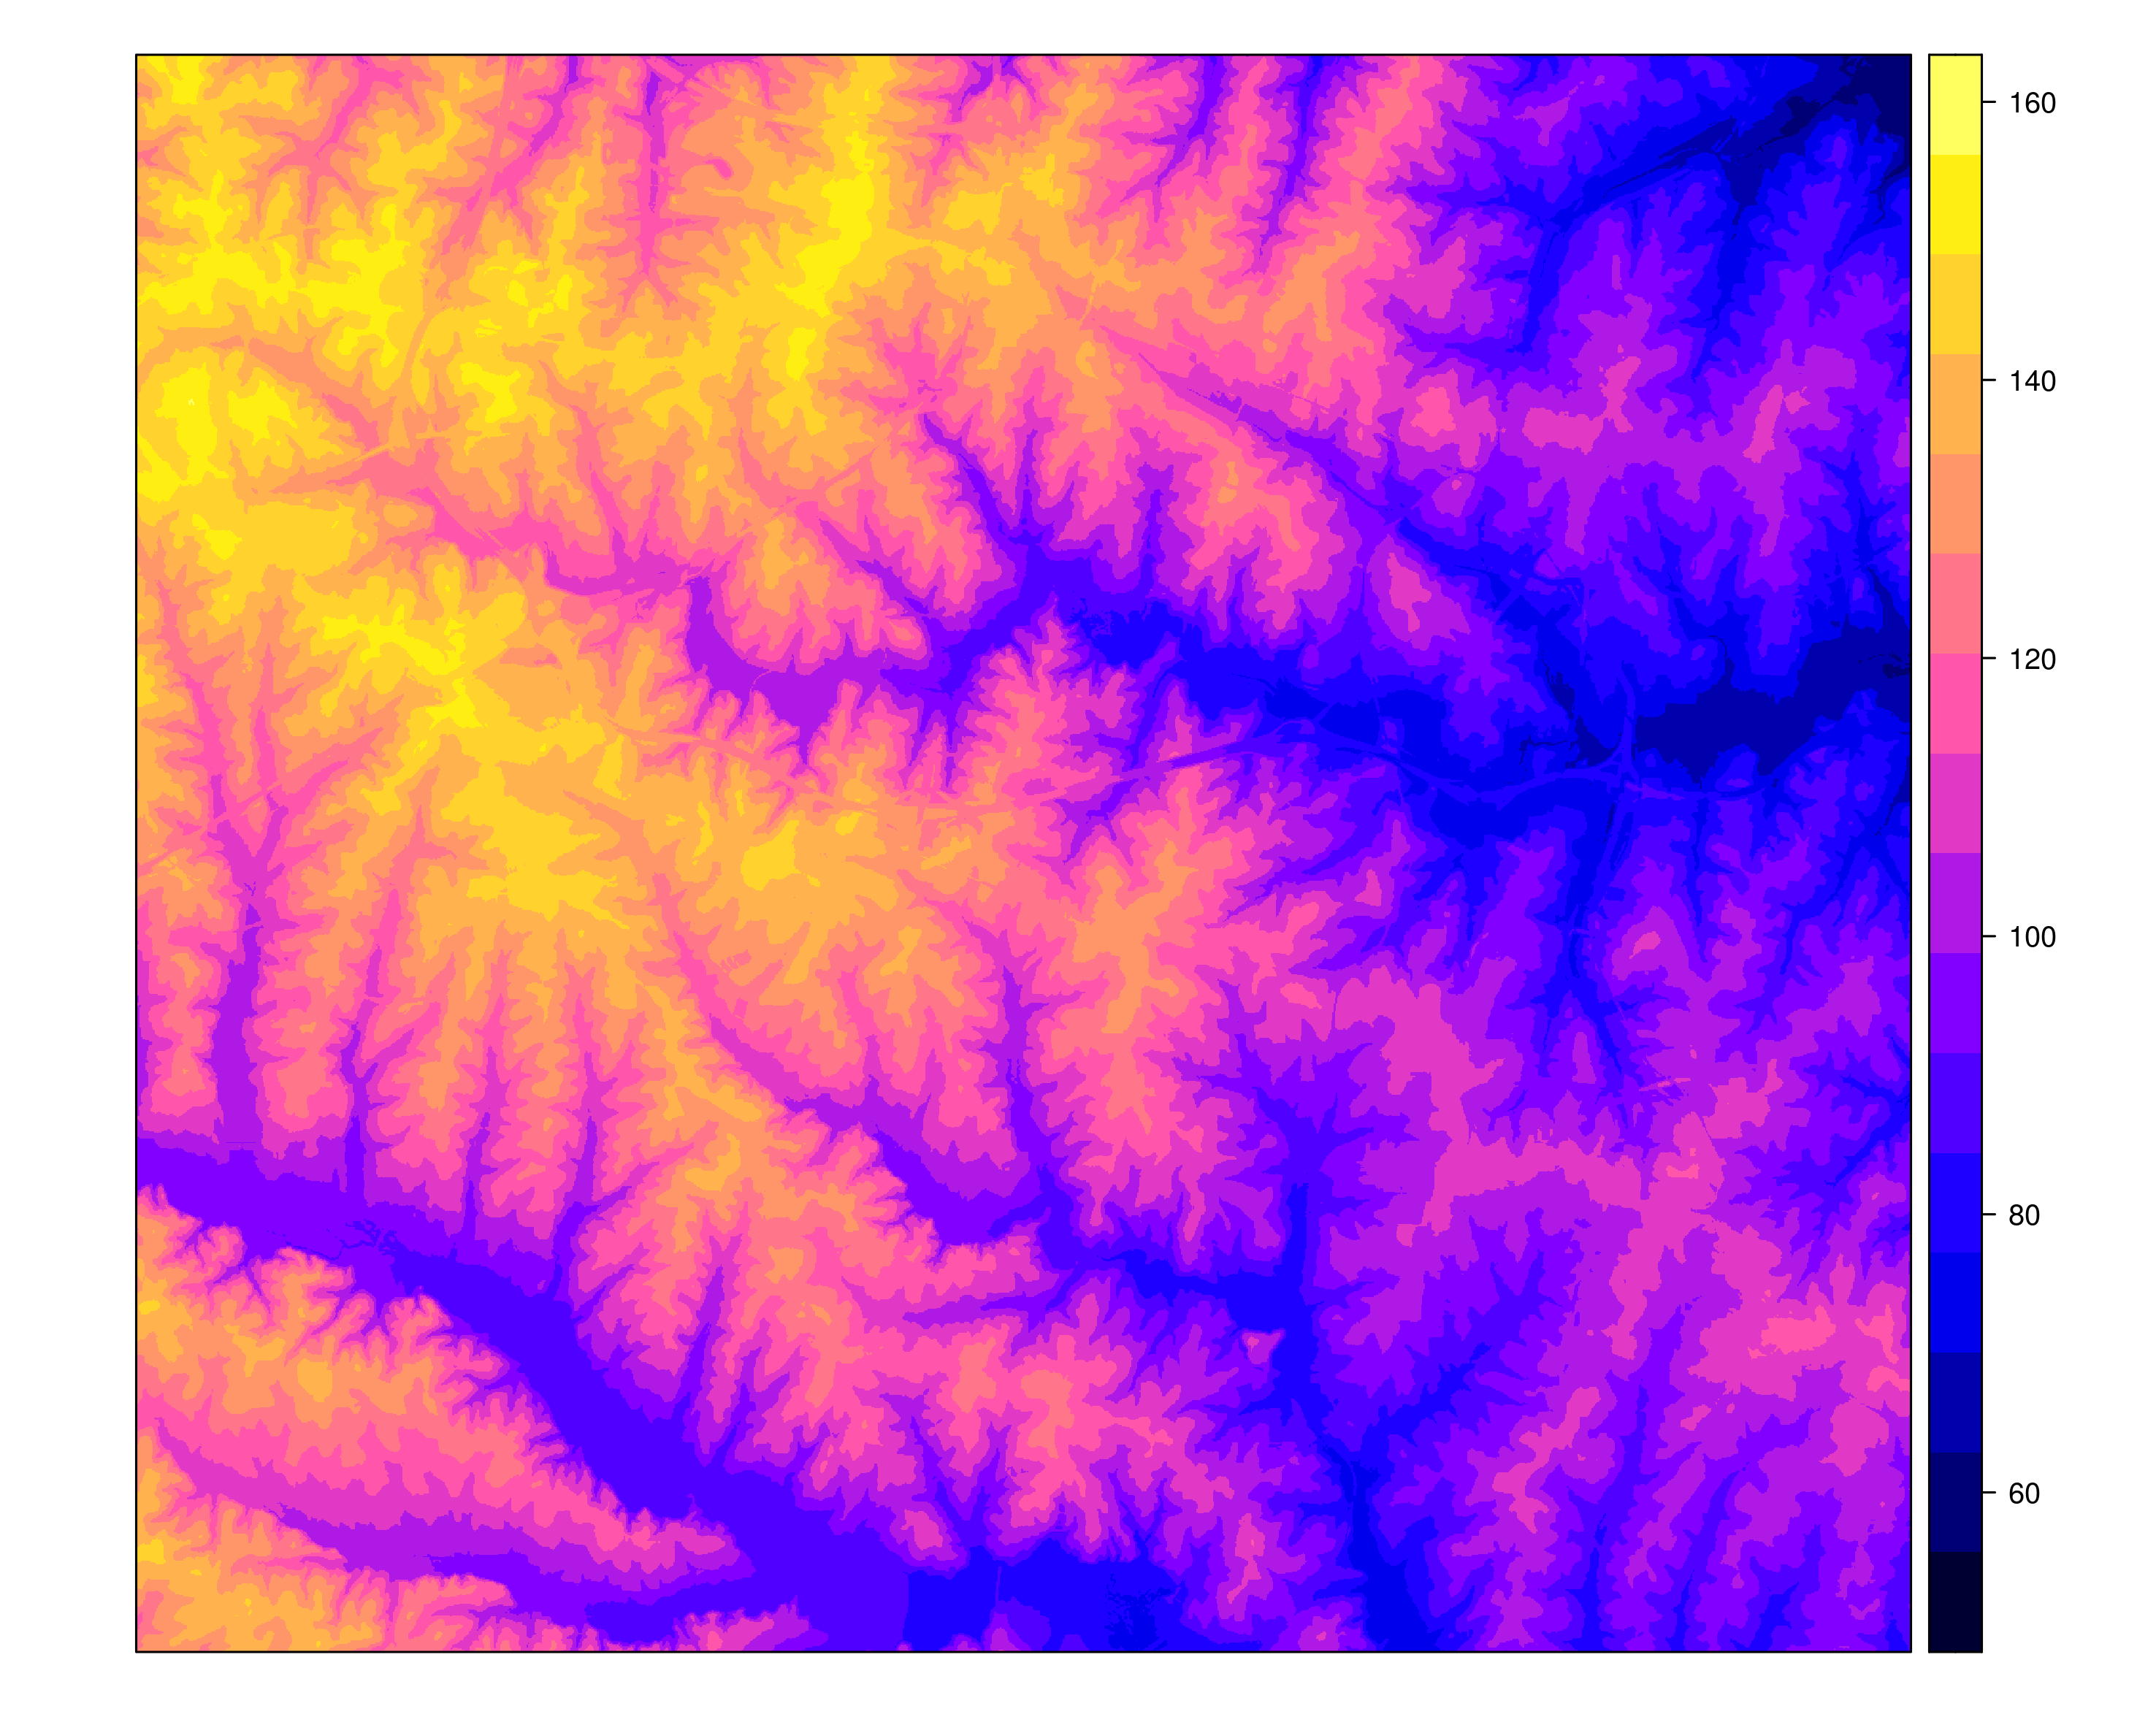
\includegraphics[width=8cm, height=8cm]{/home/jana/git/R-za-neprogramerje/Predavanje_08/grass/myplot.png}

Pregledmo vektorske podatke:

\begin{Shaded}
\begin{Highlighting}[]
\KeywordTok{library}\NormalTok{(sf)}
\end{Highlighting}
\end{Shaded}

\begin{verbatim}
## Linking to GEOS 3.6.2, GDAL 2.2.3, PROJ 4.9.3; sf_use_s2() is TRUE
\end{verbatim}

\begin{Shaded}
\begin{Highlighting}[]
\KeywordTok{use_sf}\NormalTok{()}
\KeywordTok{execGRASS}\NormalTok{(}\StringTok{"v.info"}\NormalTok{, }\DataTypeTok{map=}\StringTok{"hospitals"}\NormalTok{, }\DataTypeTok{layer=}\StringTok{"1"}\NormalTok{)}
\end{Highlighting}
\end{Shaded}

\begin{verbatim}
##  +----------------------------------------------------------------------------+
##  | Name:            hospitals                                                 |
##  | Mapset:          PERMANENT                                                 |
##  | Location:        nc_spm_08_grass7                                          |
##  | Database:        /home/jana/grass2                                         |
##  | Title:           North Carolina hospitals (points map)                     |
##  | Map scale:       1:1                                                       |
##  | Name of creator: helena                                                    |
##  | Organization:    NC OneMap                                                 |
##  | Source date:     Fri Feb  9 23:53:39 2007                                  |
##  | Timestamp (first layer): none                                              |
##  |----------------------------------------------------------------------------|
##  | Map format:      native                                                    |
##  |----------------------------------------------------------------------------|
##  |   Type of map: vector (level: 2)                                           |
##  |                                                                            |
##  |   Number of points:       160             Number of centroids:  0          |
##  |   Number of lines:        0               Number of boundaries: 0          |
##  |   Number of areas:        0               Number of islands:    0          |
##  |                                                                            |
##  |   Map is 3D:              No                                               |
##  |   Number of dblinks:      1                                                |
##  |                                                                            |
##  |   Projection: Lambert Conformal Conic                                      |
##  |                                                                            |
##  |               N:   308097.93740056    S:    20235.56440056                 |
##  |               E:    914347.8748615    W:    156998.1718615                 |
##  |                                                                            |
##  |   Digitization threshold: 0                                                |
##  |   Comment:                                                                 |
##  |                                                                            |
##  +----------------------------------------------------------------------------+
\end{verbatim}

\begin{Shaded}
\begin{Highlighting}[]
\KeywordTok{vInfo}\NormalTok{(}\StringTok{"hospitals"}\NormalTok{)}
\end{Highlighting}
\end{Shaded}

\begin{verbatim}
##      nodes     points      lines boundaries  centroids      areas    islands 
##          0        160          0          0          0          0          0 
## primitives      map3d 
##        160          0
\end{verbatim}

\begin{Shaded}
\begin{Highlighting}[]
\NormalTok{myschools <-}\StringTok{ }\KeywordTok{readVECT}\NormalTok{(}\StringTok{"hospitals"}\NormalTok{)}
\end{Highlighting}
\end{Shaded}

\begin{verbatim}
## Warning: Package rgrass7 transitioning to package rgrass for GRASS 8.
## 'readVECT' is deprecated. Use 'read_VECT' instead.
\end{verbatim}

\begin{verbatim}
## Exporting 160 features...
## v.out.ogr complete. 160 features (Point type) written to <hospitals> (GPKG
## format).
## Reading layer `hospitals' from data source 
##   `/home/jana/grass2/nc_spm_08_grass7/landsat/.tmp/masina/640.0.gpkg' 
##   using driver `GPKG'
## Simple feature collection with 160 features and 16 fields
## Geometry type: POINT
## Dimension:     XY
## Bounding box:  xmin: 156998.2 ymin: 20235.56 xmax: 914347.9 ymax: 308097.9
## CRS:           3358
\end{verbatim}

\begin{Shaded}
\begin{Highlighting}[]
\KeywordTok{print}\NormalTok{(}\KeywordTok{summary}\NormalTok{(myschools))}
\end{Highlighting}
\end{Shaded}

\begin{verbatim}
##       cat            OBJECTID           AREA     PERIMETER      HLS_       
##  Min.   :  1.00   Min.   :  1.00   Min.   :0   Min.   :0   Min.   :  1.00  
##  1st Qu.: 40.75   1st Qu.: 40.75   1st Qu.:0   1st Qu.:0   1st Qu.: 40.75  
##  Median : 80.50   Median : 80.50   Median :0   Median :0   Median : 80.50  
##  Mean   : 80.50   Mean   : 80.50   Mean   :0   Mean   :0   Mean   : 80.50  
##  3rd Qu.:120.25   3rd Qu.:120.25   3rd Qu.:0   3rd Qu.:0   3rd Qu.:120.25  
##  Max.   :160.00   Max.   :160.00   Max.   :0   Max.   :0   Max.   :160.00  
##      HLS_ID           NAME             ADDRESS              CITY          
##  Min.   :  1.00   Length:160         Length:160         Length:160        
##  1st Qu.: 40.75   Class :character   Class :character   Class :character  
##  Median : 80.50   Mode  :character   Mode  :character   Mode  :character  
##  Mean   : 80.50                                                           
##  3rd Qu.:120.25                                                           
##  Max.   :160.00                                                           
##      ZIP               COUNTY             PHONE              CANCER         
##  Length:160         Length:160         Length:160         Length:160        
##  Class :character   Class :character   Class :character   Class :character  
##  Mode  :character   Mode  :character   Mode  :character   Mode  :character  
##                                                                             
##                                                                             
##                                                                             
##    POLYGONID     SCALE       ANGLE                   geom    
##  Min.   :0   Min.   :1   Min.   :0.0000   POINT        :160  
##  1st Qu.:0   1st Qu.:1   1st Qu.:1.0000   epsg:3358    :  0  
##  Median :0   Median :1   Median :1.0000   +proj=lcc ...:  0  
##  Mean   :0   Mean   :1   Mean   :0.8313                      
##  3rd Qu.:0   3rd Qu.:1   3rd Qu.:1.0000                      
##  Max.   :0   Max.   :1   Max.   :1.0000
\end{verbatim}

Povzemanje podatkov: Naredimo tabelo kolikokrat se posamezna vrednost
pojavi.

\begin{Shaded}
\begin{Highlighting}[]
\KeywordTok{table}\NormalTok{(ncdata}\OperatorTok{$}\NormalTok{geology_30m)}
\end{Highlighting}
\end{Shaded}

\begin{verbatim}
## < table of extent 0 >
\end{verbatim}

Primerjamo z GRASS izpisom:

\begin{Shaded}
\begin{Highlighting}[]
\KeywordTok{execGRASS}\NormalTok{(}\StringTok{"r.stats"}\NormalTok{, }\DataTypeTok{flags=}\KeywordTok{c}\NormalTok{(}\StringTok{"c"}\NormalTok{, }\StringTok{"l"}\NormalTok{), }\DataTypeTok{parameters=}\KeywordTok{list}\NormalTok{(}\DataTypeTok{input=}\StringTok{"geology_30m"}\NormalTok{), }\DataTypeTok{ignore.stderr=}\OtherTok{TRUE}\NormalTok{)}
\end{Highlighting}
\end{Shaded}

\begin{verbatim}
## 217 CZfg 725562
## 262 CZlg 198684
## 270 CZig 689373
## 405 CZbg 253710
## 583 CZve 21609
## 720 CZam 4824
## 766 CZg 7074
## 862 CZam 61722
## 910 CZbg 44964
## 921 Km 12528
## 945 CZbg 9
## 946 CZam 4068
## 948 CZam 873
\end{verbatim}

Lahko narišemo ``škatle z brki'' različnih geoloških tipov po višinah

\begin{Shaded}
\begin{Highlighting}[]
\NormalTok{ncdata <-}\StringTok{ }\KeywordTok{read_RAST}\NormalTok{(}\KeywordTok{c}\NormalTok{(}\StringTok{"geology_30m"}\NormalTok{, }\StringTok{"elevation"}\NormalTok{), }\DataTypeTok{cat=}\KeywordTok{c}\NormalTok{(}\OtherTok{TRUE}\NormalTok{, }\OtherTok{FALSE}\NormalTok{))}
\end{Highlighting}
\end{Shaded}


\begin{verbatim}
## Warning in .read_rast_non_plugin_ng(vname = vname, cat = cat, NODATA = NODATA, :
## non-unique category labels; category number appended
\end{verbatim}

\begin{Shaded}
\begin{Highlighting}[]
\NormalTok{da <-}\StringTok{ }\KeywordTok{data.frame}\NormalTok{(}\DataTypeTok{elevation =}\NormalTok{ ncdata}\OperatorTok{$}\NormalTok{elevation, }\DataTypeTok{geology_30m =}\NormalTok{ ncdata}\OperatorTok{$}\NormalTok{geology_30m)}
\KeywordTok{library}\NormalTok{(ggplot2)}
\KeywordTok{ggplot}\NormalTok{(da, }\KeywordTok{aes}\NormalTok{(}\DataTypeTok{x =}\NormalTok{ geology_30m, }\DataTypeTok{y=}\NormalTok{ elevation)) }\OperatorTok{+}\StringTok{ }\KeywordTok{geom_boxplot}\NormalTok{()}
\end{Highlighting}
\end{Shaded}

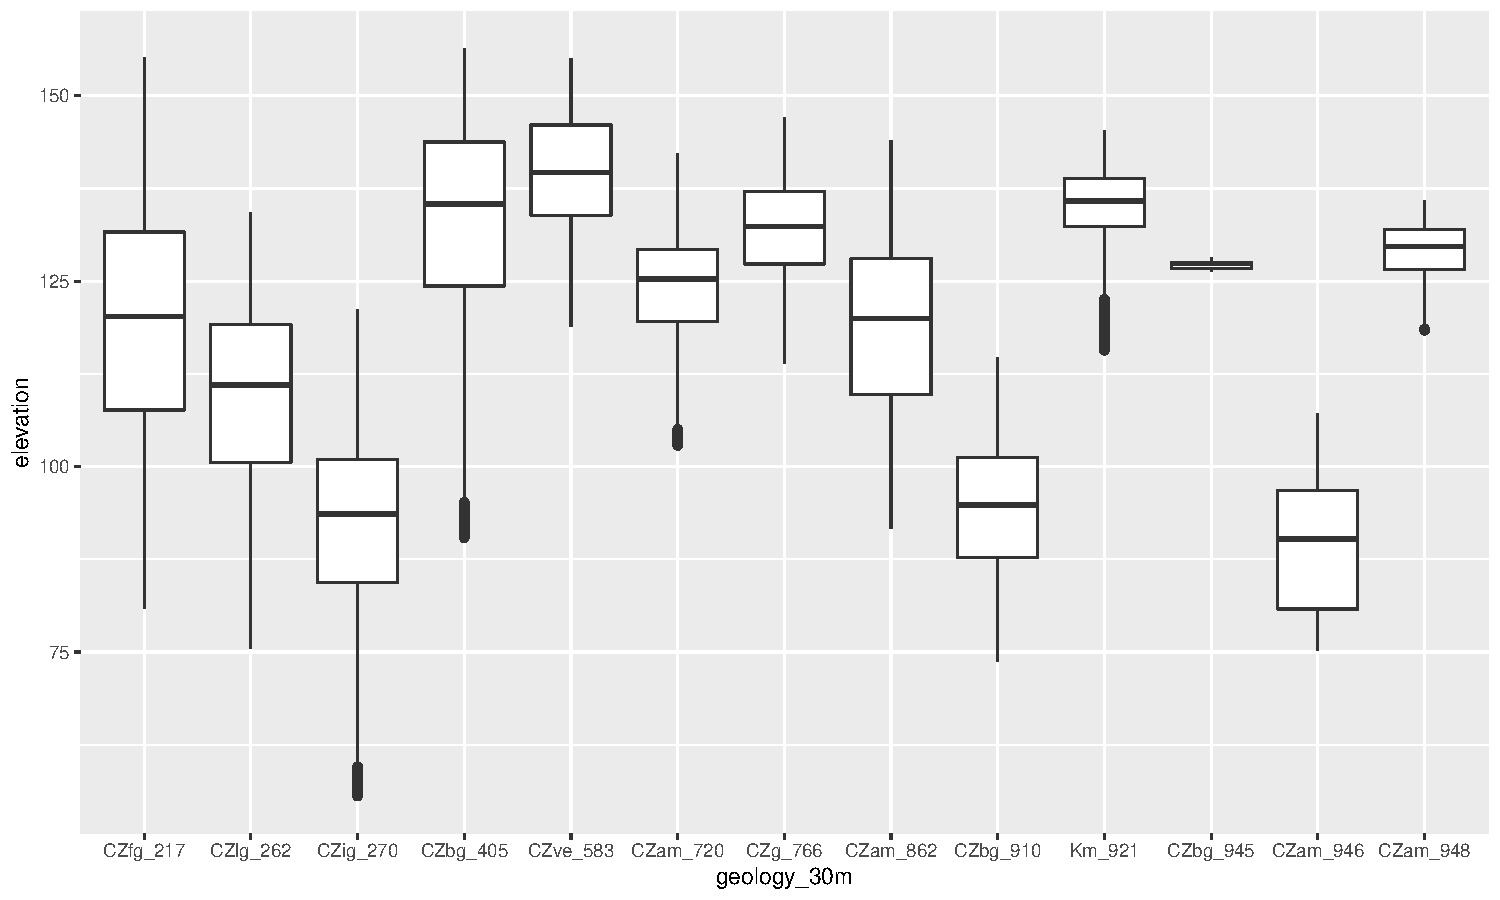
\includegraphics{/home/jana/git/R-za-neprogramerje/Predavanje_08/grass/box.pdf}

\end{document}
